\chapter{Método propuesto}

En el capítulo 3 se describieron los principales retos del perfilado de autor y las principales características de los métodos existentes para el aumento de datos en la clasificación de textos. Observando las características de los métodos de aumento de datos existentes, en este capítulo se describen los métodos propuestos para hacer el aumento de datos, para tareas relacionadas al perfilado de autor. 

Como se mostró en el capítulo anterior, existen numerosas técnicas de aumento de datos, sin embargo, no todas son generalizables o escalables, además de que, en el caso de perfilado de autor se desea conservar tanto el estilo como el contenido de un texto, considerando el estilo como la forma o modo de expresar el contenido, siendo el contenido el tema o mensaje a transmitir. De ahí que la mejor forma de hacer el aumento de datos en esta tarea es mediante el parafraseo humano, pero debido a su costo, no siempre es posible. En cambio, podemos apoyarnos de técnicas automáticas para aproximarse al parafraseo \citep{androutsopoulos2010survey}. Cabe mencionar que el resultado de estos métodos automáticos difícilmente obtiene paráfrasis de las oraciones originales. 

El aumento de datos propuesto busca conservar el estilo de las frases originales, y con ellas incrementar el conjunto original. Los métodos desarrollados en este trabajo tienen dos pasos generales que se describen a continuación: 

\begin{enumerate}
    \item \textbf{Selección de palabras a reemplazar}: El primer paso consiste en identificar el subconjunto de palabras a reemplazar. Dos criterios son relevantes en esta etapa: (i) la importancia de la palabra en la estructura de la frase, es decir, no se tiene el mismo efecto si se reemplaza una palabra de contenido que una palabra funcional; (ii) la cantidad de palabras a reemplazar, dado que se desea conservar la misma interpretación de la frase original, el número de reemplazos deberá controlarse.  
    \item \textbf{Reemplazo de palabras seleccionadas}: Una vez determinado el subconjunto de palabras a reemplazar, se deberán identificar nuevas palabras que no alteren significativamente el sentido de la frase original. Para esto se recurre a un recurso externo, tal como un tesauro, un diccionario, o incluso a modelos distribucionales de vectores de palabras.
     Después de identificar las palabras sustitutas se reconstruye la secuencia manteniendo el orden original para formar la nueva secuencia aumentada. 
\end{enumerate}

Es importante mencionar que los métodos de aumento de datos propuestos son independientes del conjunto de datos. De hecho, no se utiliza la oración como unidad básica, sino una secuencia de palabras de longitud fija. De esta forma el conjunto original es fragmentado obteniendo un conjunto $S$ de secuencias de tamaño fijo. Los métodos de aumento de datos propuestos recorren, este conjunto $S$, obteniendo una nueva aproximación $\hat{s}$ para cada secuencia $s$ en $S$. El nuevo conjunto $\hat{S}$ obtenido se agrega al conjunto original $S$ aumentando el conjunto de entrenamiento. Este proceso sobre el conjunto original $S$ puede repetirse $n$ veces, incrementando sucesivamente el conjunto de entrenamiento para la clase de interés.
En el caso particular de este trabajo, nos interesa analizar el aumento de datos en situaciones con colecciones de datos desbalanceadas, de ahí que el aumento se datos se aplica a la clase minoritaria, es decir, la clase de interés. 

\section{Selección de palabras a reemplazar}

El primer punto bajo este proceso es el cálculo del número de palabras a reemplazar. Para esto, se retomó el criterio presentado en \citep{zhang2015character}. El número de palabras a reemplazar $r$ se selecciona mediante un muestreo aleatorio de una distribución de probabilidad geométrica. 

Una función de probabilidad geométrica es la función de probabilidad del número $X$ del ensayo de Bernoulli de obtener éxito, soportado en el conjunto de los números naturales. Una distribución geométrica da la probabilidad de que la primera ocurrencia de éxito requiere de $k$ ensayos independientes, cada uno con una probabilidad de éxito $p$. Si la probabilidad de éxito de cada ensayo es $p$, entonces la probabilidad de que en el $k$-ésimo ensayo, de $k$ ensayos, sea el primer éxito es representada en la ecuación \ref{eq:geom}.

\begin{equation} \label{eq:geom}
    Pr(X=k)=(1-p)^{k-1}p
\end{equation}

Por lo tanto, la aleatoriedad del número $r$ es controlada mediante la modificación del parámetro $p$ como se representa en figura \ref{fig:geom}. Como puede verse en dicha figura, mientras menor sea el valor de $p$ se modificará un mayor número de palabras, agregando una mayor diversidad y consecuentemente incrementando la probabilidad de alterar el significado original. 
\begin{figure}[ht]
    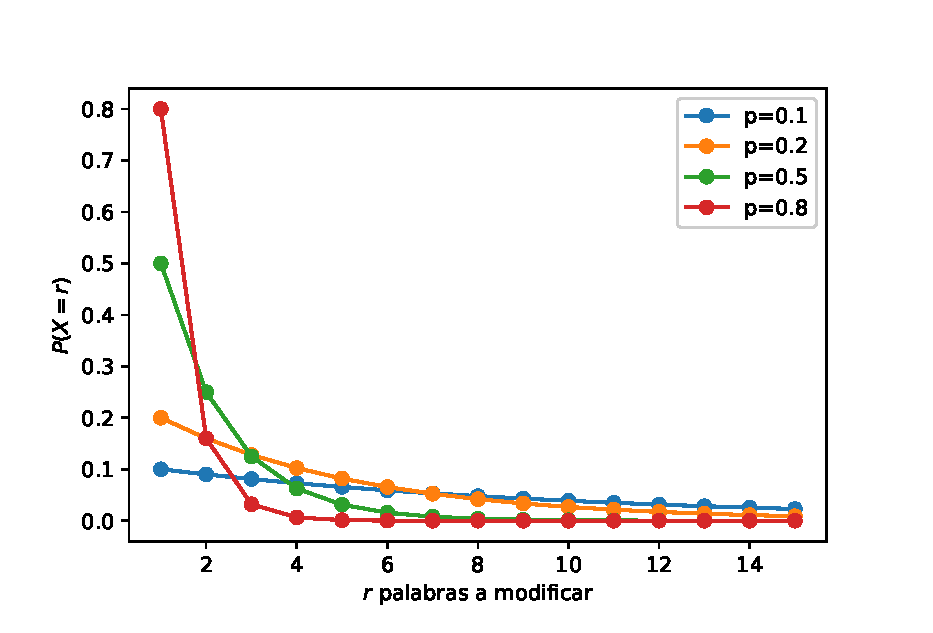
\includegraphics[width=\textwidth]{sections/figures/geometric_pmf.eps}
    \caption{Función de masa para la distribución geométrica con diferentes valores de probabilidad.}
    \label{fig:geom}
\end{figure}

\subsection{Etiquetado de partes de la oración}
El proceso de selección debe cuidar la modificación de ciertas partes de la oración, por un lado, evitar perder la interpretación original y por otro intentar conservar el estilo de la frase original. Por tal motivo, cada frase es etiquetada asignando a cada palabra su etiqueta POS (\textit{part of speech}) correspondiente. La tabla \ref{table:pos} muestra un ejemplo del etiquetado aplicado. Gracias al etiquetado, las palabras a reemplazar solo son aquellas que están más fuertemente asociadas al contenido de la frase, es decir, solo se seleccionan aquellas palabras con funciones gramaticales de: sustantivo, adjetivo, verbo y/o adverbio.


\begin{table}[h]
\caption{Ejemplo de etiquetado de partes de la oración.} \label{table:pos}
\begin{center}
\begin{tabular}{lllllll}
\hline
\textbf{Secuencia} & \textit{I} & \textit{am} & \textit{running} & \textit{out} & \textit{of} & \textit{ideas} \\ \hline
Etiqueta           & PRP        & VBP         & VBG              & IN           & IN          & NNS            \\ \hline
Equivalencia       & Pronombre  & Verbo       & Verbo            & Preposición  & Preposición & Sustantivo     \\ \hline
\end{tabular}
\end{center}
\end{table}

\subsection{Exclusión de palabras importantes}

Además de las palabras funcionales, también es deseable mantener palabras que aportan información para la tarea de clasificación que se desea realizar, por lo tanto, la primera propuesta consiste en evitar seleccionar, entre las palabras a reemplazar, aquellas palabras dependientes a la clase del documento. 

Para este proceso, recurrimos a la técnica de selección de características conocida como prueba de independencia $\chi^2$ (chi cuadrada). En estadística, la prueba $\chi^2$ es aplicada para comprobar la independencia de dos eventos, donde los eventos $A$ y $B$ son definidos a ser independientes si $P(AB)= P(A)P(B)$ o, equivalente, $P(A|B)=P(A)$ y $P(B|A)=P(B)$. En la selección de características para la clasificación de textos, los dos eventos son: \textit{ocurrencia del término} y \textit{ocurrencia de la clase}. Posteriormente se ordenan los términos de mayor a menor respecto a la ecuación \ref{eq:chi2}.

\begin{equation}
    \label{eq:chi2}
    \chi^2(D, t, c)= \sum_{e_t \in {0,1} }^{} \sum_{e_c \in {0,1} }^{} \frac{(N_{e_t e_c} - E _{e_t e_c})^2}{E_{e_t e_c}}
\end{equation}

El término $e_t$ indica la ausencia o presencia del término $t$ en el documento, similarmente el término $e_c$ indica si el documento se encuentra en la clase $c$. $N$ es la frecuencia observada en $D$ y $E$ es la frecuencia esperada. $\chi^2$ mide por cuanto los conteos esperados $E$ y los conteos observados $N$ se desvían de cada uno. Un valor alto de $\chi^2$ indica que la hipótesis de independencia, la cual implica que los conteos esperados y observados son similares, es incorrecta. Si los dos eventos son dependientes, entonces la ocurrencia del término hace la ocurrencia de la clase más probable (o menos probable), entonces el término debería ser seleccionado como relevante.

A través de este método se identifican todas aquellas palabras dependientes de la clase y, por ende, de relevancia para la tarea de clasificación. Dada la importancia de estas palabras se evitará reemplazarlas, excluyéndolas del proceso de selección de palabras a reemplazar.

\section{Reemplazo de palabras seleccionadas}

Una vez identificadas las palabras a reemplazar, el siguiente paso es, mediante la consulta de alguna fuente de conocimientos externa, buscar palabras candidatas similares a la palabra que se desea reemplazar. En \citep{zhang2015character} proponen consultar un tesauro con el objetivo de obtener los sinónimos de una palabra, sin embargo, el vocabulario contenido en el tesauro puede ser muy limitado o demasiado formal para el contexto del texto a aumentar. 

Una alternativa es buscar palabras similares a través de representaciones distribucionales de las palabras. La idea general de las representaciones distribucionales es codificar los \textit{tokens} de un vocabulario de tamaño finito $|V|$, en un vector que lo represente en espacio de palabras. La principal intuición de este enfoque es que deberá existir algún espacio $n$-dimensional, tal que $n<|V|$, donde codificar toda la semántica de un idioma. Cada dimensión codificará algún tipo de información, por ejemplo: las dimensiones semánticas podrían indicar el tiempo de conjugación (pasado, presente o futuro), de conteo (singular o plural) y género (masculino o femenino). En la subsección 2.2.4 se describen los modelos del estado del arte que siguen esta metodología.

El presente trabajo explora dos enfoques utilizando este recurso, la siguiente sección explica ambos enfoques.

\subsection{Similitud relacional}

Las representaciones distribucionales calculadas utilizando redes neuronales son muy interesantes debido a que los vectores aprendidos codifican muchas regularidades lingüísticas y patrones \citep{mikolov2013distributed}. Una de estas regularidades es la sinonimia y puede ser recuperada mediante alguna medida de distancia entre una palabra objetivo $w$ y el resto del vocabulario $V$. Esto se puede observar en la figura \ref{fig:word_plot}, en la cual se proyectan los vectores correspondientes a las palabras en un plano de dos dimensiones. En la figura, se observan las distancias entre palabras relacionadas con la palabra \textit{depresión} las cuales aparecen cercanas a una palabra, cuyo significado es más contrastante como la palabra \textit{feliz}. 

\begin{figure}[!hbt]
    \centering
  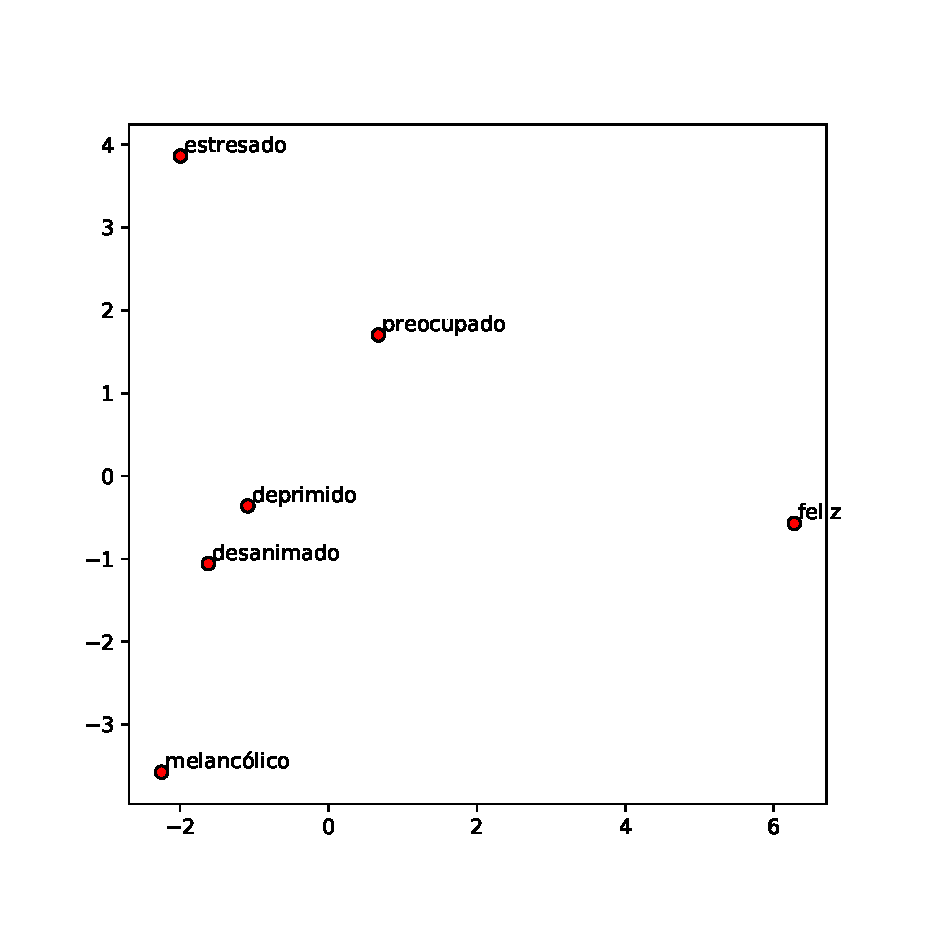
\includegraphics[scale=0.7]{sections/figures/word_plot.eps}
    \caption{Ejemplo comparando las distancias entre las proyecciones de los vectores de  palabras relacionadas a la palabra \textit{depresión} en contraste a la palabra \textit{feliz}.}
    \label{fig:word_plot}
\end{figure}

\subsubsection{Reemplazo por similitud relacional coseno}

La primera propuesta de reemplazo utiliza las representaciones distribucionales para reemplazar una palabra en una secuencia, por una palabra similar o altamente relacionada (i.e., aparecen en contextos similares). Para realizar esto se recupera el vector de la palabra a reemplazar de un modelo preentrenado de vectores de palabras y se calcula la distancia respecto a cada vector (representación de una palabra) en el modelo preentrenado. En este caso, hemos usado la medida de similitud coseno, véase la ecuación \ref{eq:coseno}. Esta ecuación indica que para obtener la distancia coseno de dos vectores de palabras se debe hacer un producto punto entre los vectores ($\vec{w}$, $\vec{v}$) y dividir el resultado por la multiplicación de la magnitud de los mismos.

\begin{equation}
\label{eq:coseno}
    cos(\vec{w},\vec{v})=\frac{\vec{w} . \vec{v}}{||\vec{w}||||\vec{v}||} = \frac{\sum_{i=1}^{n}w_i v_i}{\sqrt{\sum_{i=1}^{n}(w_i)^2} \sqrt{\sum_{i=1}^{n}(v_i)^2} }
\end{equation}

Específicamente para encontrar el conjunto de palabras candidatas $W$, dada una palabra $w$ se buscan las $k$ palabras más similares a $w$ de acuerdo con la ecuación \ref{eq:cosmax}.

\begin{equation}
    \label{eq:cosmax}
    argmax_{v \in V} (cos(\vec{w}, \vec{v}))
\end{equation}

Donde $\vec{v}$ es la representación vectorial de cada palabra en el vocabulario $V$ de vectores preentrenados y $\vec{w}$ es la representación vectorial de la palabra a sustituir. Una alta similitud coseno (cercana a 1) significa que los vectores comparten una dirección muy similar y por lo tanto hay una mayor probabilidad que las palabras sean utilizadas en los mismos contextos. En la tabla \ref{table:ejemplos_xi} se muestra el ejemplo de una secuencia, aumentada mediante este método, las palabras en negritas no se modifican debido a que son palabras con alta puntuación $\chi^2$ y en cursiva son resaltadas las palabras que se reemplazaron de la secuencia original. En el ejemplo la palabra \textit{morning} tiene como palabras candidatas las palabras:\textit{ sunday, afternoon y evening}. Aunque estas palabras no representan sinónimos de \textit{morning}, si conservan la misma etiqueta POS manteniendo el estilo de la secuencia original. 

\begin{table}[hbt!]
\caption{Ejemplos del aumento de datos, para el método con restricción $\chi^2$ y sustitución por similitud relacional.} 
\label{table:ejemplos_xi}
\centering
\begin{tabular}{ll}
\hline
                  & \textbf{Secuencia}                                                        \\ \hline
\textbf{Original} & \textbf{just} waking up every morning and \textbf{talking} to \textbf{my} gf \\ \hline
Aumentada         & just waking up every \textit{sunday} and talking to my gf \\ \hline
Aumentada         & just waking up every \textit{afternoon} and talking to my gf \\ \hline
Aumentada         & just \textit{woke} up every \textit{evening} and talking to my gf  \\ \hline
\end{tabular}

\end{table}


\subsubsection{Reemplazo por relaciones equivalentes}
Una de las características deseables en el aumento de datos es agregar un grado de diversidad o variabilidad en nuestros datos, sin embargo, al utilizar las representaciones distribucionales encontramos que las palabras con alta similitud coseno a una palabra, son por lo general variaciones pequeñas de esta misma palabra, por ejemplo, en la figura \ref{fig:analogia} lo más cercano a \textit{llorar} es \textit{llorando}. En este caso notamos que la diversidad deseada no se logra. 
Otro problema encontrado al calcular la similitud coseno entre dos palabras, dados sus vectores, es encontrar que palabras como \textit{llorar} y \textit{reir} suelen ser similares. Esto sucede porque ambas palabras ocurren en contextos de uso similares. Sin embargo, no deseamos hacer este tipo de sustituciones ya que sustituir una palabra por su antónimo (en lugar de un sinónimo) podría causar que la etiqueta original del documento se pierda.
\begin{figure}[!hbt]
\centering
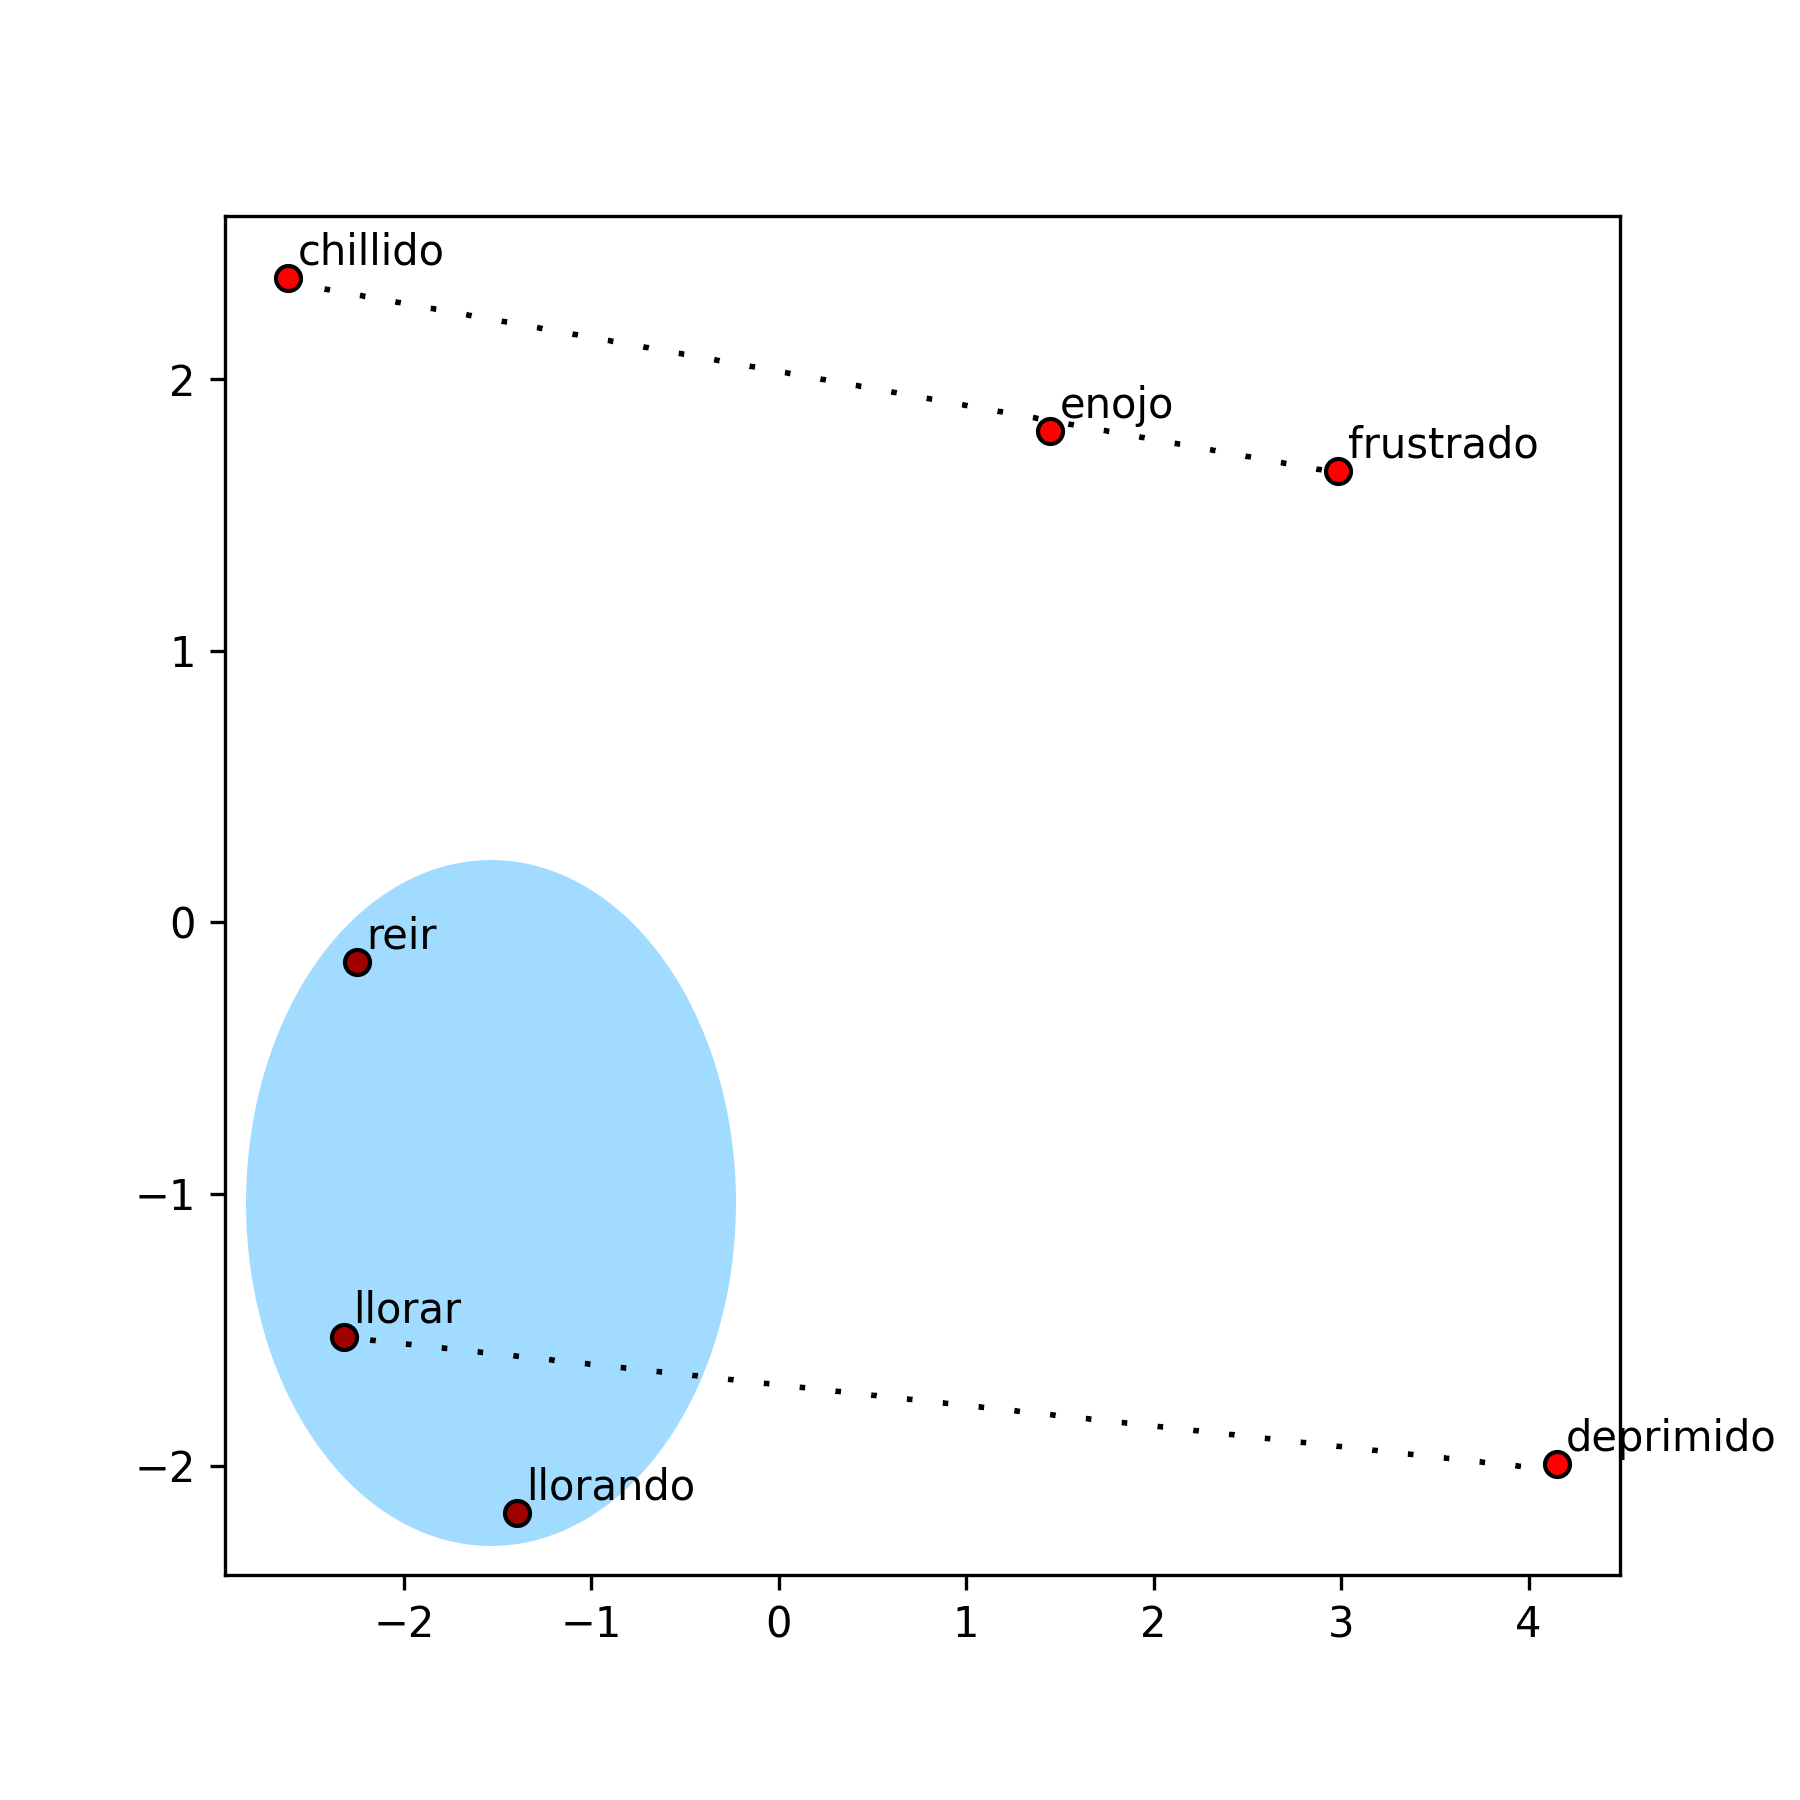
\includegraphics[width=0.7 \textwidth]{sections/figures/analogia.png}
\caption{Palabras que ocurren en contextos de uso similares tienen una similitud relacional alta, incluyendo el caso de antónimos, por ejemplo \textit{llorar} vs \textit{reír} }
\label{fig:analogia}
\end{figure}

Para resolver este problema, explotamos la similitud relacional entre pares de palabras. Por ejemplo, al recuperar las palabras más similares a la palabra \textit{llorar}, encontramos: reír y llorando. Si sumamos el vector de la palabra \textit{llorar} con el vector de la palabra \textit{frustrado} podemos encontrar entre las palabras más cercanas: \textit{chillido} y \textit{enojo}, tal como se muestra en la figura \ref{fig:analogia}. De esta forma, mediante la aritmética de vectores podemos descubrir relaciones no tan obvias, y con ello crear una mayor diversidad en el vocabulario. Estas relaciones han sido previamente demostradas en \citep{mikolov2013linguistic}, junto con relaciones como singular - plural, adjetivos posesivo - no posesivo, base - comparativo, base - superlativo. Por  supuesto, se trata de una aproximación con la cual se ha alcanzado exactitudes de hasta un 41\%. 

En un contexto de aumento de datos asumimos que existe una relación entre la etiqueta de la clase y las palabras de una secuencia en un documento de esa clase. Para observar esta relación empleamos pares de palabras, intentando identificar analogías. Por ejemplo, se busca encontrar un segundo par de palabras que presente una relación análoga entre las palabras \textit{deprimido} (etiqueta de la clase) y \textit{llorar} (palabra de una secuencia perteneciente a la clase). En este caso suponemos que existe una relación entre \textit{deprimido} y \textit{llorar}; el siguiente paso es buscar una relación similar entre un sinónimo de \textit{deprimido}, puede ser \textit{frustrado}, y una palabra $v$ que desconocemos. Estas relaciones se muestran en la figura \ref{fig:analogia} mediante una línea punteada. 

 \begin{equation}
    \label{eq:grl_ejemplo}
     v \approx  llorar-deprimido+frustrado
 \end{equation}


De manera general para el aumento de datos proponemos expresar una analogía de la forma `` $w_{label}$ es a $w$ como $w_{syn}$ es a $v$", resolviendo la ecuación \ref{eq:grl_analogia} mediante aritmética de vectores.

 \begin{equation}
    \label{eq:grl_analogia}
    \vec{v} \approx \vec{w}-\vec{w_{label}}+\vec{w_{syn}}
\end{equation}
 
La ecuación \ref{eq:grl_ejemplo} resulta de sustituir en la ecuación \ref{eq:grl_analogia} las palabras involucradas para el aumento de datos. 
Siendo $\vec{w}$, $\vec{w_{label}}$  y $\vec{w_{syn}}$ las representaciones vectoriales de la palabra $w$ a reemplazar, la etiqueta de la clase a aumentar $w_{label}$ y un sinónimo de la etiqueta de la clase a aumentar $w_{syn}$. El vector $\vec{v}$ es la representación vectorial de la palabra a encontrar. Se busca que la palabra $v$ sea muy similar a $w$ pero orientada en el contexto del sinónimo $w_{syn}$. Es decir, el objetivo principal es encontrar palabras candidatas $v$ que comparten la misma relación reflejada entre \textit{llorar - deprimido} pero no necesariamente similar a \textit{llorar}.

 La ecuación \ref{eq:grl_analogia} es una forma directa para resolver preguntas de analogía. En \citep{mikolov2013linguistic}, propusieron este método nombrándolo método de compensación de vectores, en este método se asume que las relaciones semánticas entre palabras están presentes como una compensación de vectores, así que, en el espacio de características, todos los pares de palabras compartiendo una relación en particular están relacionadas por la misma constante de compensación. La variable $\vec{v}$ es la representación del espacio continuo de la palabra que esperamos sea la mejor respuesta. Claramente no existe ninguna palabra en la posición exacta, así que se busca la palabra cuyo vector tenga la mayor similitud coseno a $\vec{v}$. Resultando en:

\begin{equation}
\label{eq:3cosadd}
    arg max_{\vec{v}\in V}( cos (\vec{v}, \vec{w}-\vec{w_{label}}+\vec{w_{syn}}))
\end{equation}

Antes de aplicar la operación en \ref{eq:3cosadd}, todos los vectores son normalizados al vector unitario. Bajo esta normalización, dicha ecuación se puede expandir como en \ref{eq:3cosadd2}

\begin{equation}
\label{eq:3cosadd2}
    arg max_{\vec{v}\in V}( cos(\vec{v}, \vec{w}) - cos(\vec{v}, \vec{w_{label}}) + cos(\vec{v}, \vec{w_{syn}}) )
    \end{equation}

El objetivo anterior busca encontrar una palabra similar a $w$ (la palabra que deseamos reemplazar), diferente de $w_{label}$ (la etiqueta de la clase a aumentar) y similar a $w_{syn}$ (un sinónimo de la etiqueta a aumentar). Al maximizar este objetivo \citep{mikolov2013distributed} comprobó que se puede recuperar hasta un 53\% de las analogías en el conjunto de datos MSR\footnote{research.microsoft.com/en-us/projects/rnn/}. Aun así, \citep{levy2014linguistic} encontró que la formulación en \ref{eq:3cosadd2} permite que un término suficientemente grande domine la expresión y como consecuencia obtener resultados incorrectos, para alcanzar un mejor balance entre los diferentes aspectos de similitud, propusieron la ecuación 3COSMUL ( \ref{eq:3cosmul}). Esta fórmula amplifica las diferencias entre pequeñas cantidades y las reduce entre las grandes. Mediante esta fórmula se logro recuperar el 59\% de las analogías en el conjunto MSR.

\begin{equation}
    \label{eq:3cosmul}
    arg max_{\vec{v}\in V} \frac{ cos(\vec{v}, \vec{w}) cos(\vec{v}, \vec{w_{sym}})}
    { cos(\vec{v}, \vec{w_{label}})+ \epsilon}
\end{equation}

Bajo este nuevo escenario, primero se obtiene la similitud de la palabra $w$ a ser reemplazada y una palabra $v$ en el vocabulario, el resultado es multiplicado por la similitud de la palabra $v$ y un sinónimo de la etiqueta de la clase a aumentar $w_{syn}$. Con esto se espera amplificar la similitud entre $v$ y la palabra a reemplazar $w$ por la magnitud de la similitud entre $v$ y $w_{syn}$. El denominador busca incrementar el resultado anterior si existe disimilitud entre $v$ y la etiqueta $w_{label}$ de la palabra a aumentar. 
Finalmente, sustituyendo las representaciones vectoriales de $v$ para cada palabra en el vocabulario $V$, $w$, $w_{label}$ y $w_{syn}$ en la formula \ref{eq:3cosmul} obtenemos las palabras candidatas $W$ con mayor puntuación. Antes de obtener el resultado de \ref{eq:3cosmul}, las similitudes coseno son transformadas en el rango [0,1] utilizando $\frac{x+1}{2}$ y $\epsilon$ es un número muy pequeño usado para evitar la división por cero.

En la tabla \ref{table:ejemplos_equiv}, se presenta un ejemplo de este método de aumento, el cual hemos nombrado de \textbf{reemplazo por relaciones equivalentes}.
En la primera columna se indica la etiqueta de la clase a aumentar \textit{depressed} y sus sinónimos: \textit{anxious, frustrated, unhappy, despondent y discouraged}; por cada sinónimo se obtiene una secuencia aumentada.

\begin{table}[hbt!]
\caption{Ejemplos del aumento de datos para el método basado en reemplazo por relaciones equivalentes.} 
\label{table:ejemplos_equiv}
\begin{center}
\resizebox{\columnwidth}{!}{%

\begin{tabular}{ll}
\hline
 & \textbf{Secuencia}                                        \\ \hline
\textbf{Original}                                                & oh man this sucks it maybe looks funny from outside but it just looks like hell from here              \\ \hline
\begin{tabular}[c]{@{}l@{}}depressed-\\ anxious\end{tabular}     & oh man this sucks it maybe look funny from outside but it just \textit{looked} like \textit{wait} from here              \\ \hline
\begin{tabular}[c]{@{}l@{}}depressed-\\ frustrated\end{tabular}  & oh man this suck it \textit{perhaps} looks \textit{stupid} from outside but it just looks like hell from here            \\ \hline
\begin{tabular}[c]{@{}l@{}}depressed-\\ unhappy\end{tabular}     & oh \textit{woman }this sucks it maybe \textit{looking} funny from outside but it just looks like hell from here          \\ \hline
\begin{tabular}[c]{@{}l@{}}depressed-\\ despondent\end{tabular}  & oh man this \textit{pisses} it though looks \textit{humourous }from outside but it just \textit{dashing} like \textit{purgatory }from here \\ \hline
\begin{tabular}[c]{@{}l@{}}depressed-\\ discouraged\end{tabular} & oh \textit{god} this \textit{sucked} it \textit{anyway} \textit{seems humorous} from outside but it just think \textit{like bother} from here       \\ \hline
\end{tabular}


}

\end{center}
\end{table}


\subsubsection{Reemplazo por relaciones contrarias}

En escenarios desbalanceados el aumento de datos puede llevarnos a un sobremuestreo de la clase minoritaria, generalmente la clase de interés. Los métodos presentados anteriormente fueron diseñados para aumentar esta clase minoritaria (a la cual también nos referimos como clase positiva). Sin embargo, una desventaja de hacer esto es que el modelo de aprendizaje se restringe al vocabulario de la clase positiva lo que provoca un sobreajuste. En un intento de contrarrestar esta situación, se propone un método que incorpora documentos seleccionados de la clase negativa a la clase positiva. Por supuesto, para ello es necesario realizar una transformación de las instancias negativas.

Para llevar a cabo esta transformación adaptamos el método propuesto por \citep{zhang2019integrating}. En dicho método se aborda el problema de  \textit{zero-shot text classification}, en esa situación se toma un documento de una clase etiquetada y lo \textit{traduce} para considerarlo como instancia de una clase totalmente nueva. Este método no tiene ninguna restricción respecto sobre las palabras a reemplazar, en nuestro caso hemos incluido un criterio de selección para guiar la generación de los nuevos documentos los cuales servirán para aumentar el conjunto de la clase de interés.   

La idea básica de la transformación recae en el mismo método visto en la sección anterior. Sin embargo, los pares de palabras usadas para representar la analogía son escogidas para identificar palabras con una relación opuesta o \textit{contraria}. Por ejemplo, en el caso de la tarea de detección de depresión, asociaremos la palabra \textit{``feliz"} como representativa de la clase \textit{no deprimidos}  y la palabra \textit{``deprimido"} para la clase \textit{deprimidos}. Ahora bien, reemplazaremos palabras de documentos de la clase \textit{no deprimidos} por palabras que presentan la relación opuesta deseada, la cual es guiada por el par de palabras \textit{feliz} vs \textit{deprimido}. 

En la ecuación \ref{eq:contraria} se asume que existe una relación entre la palabra a reemplazar (novia) y la etiqueta de la clase no depresiva (feliz), buscamos una palabra $v$ que comparte una relación similar entre (novia) y la etiqueta que deseamos aumentar (feliz).

\begin{equation}
    \label{eq:contraria}
    v \approx novia - feliz + deprimido.
\end{equation}
Sustituyendo las palabras de \ref{eq:contraria}: novia, feliz y deprimido por su representación vectorial en \ref{eq:3cosmul} como $\vec{w}$, $\vec{w_{label}}$ y $\vec{w_{syn}}$ respectivamente.
 

La tabla \ref{table:ejemplos_contraria} presenta ejemplos del aumento basado en relaciones contrarias, las palabras relacionadas con un contexto feliz, son llevadas a un contexto contrario. Por ejemplo, el verbo \textit{``talked"} es reemplazado por \textit{``complained"} y \textit{``bothered"}. Similar al método anterior se utilizan los sinónimos de la palabra \textit{depressed} para el aumento.

\begin{table}[hbt!]
\caption{Ejemplos del aumento de datos para el método basado en relaciones opuestas.} 
\label{table:ejemplos_contraria}
\begin{center}

\begin{tabular}{ll}
\hline
\rowcolor[HTML]{EFEFEF} 
\textbf{Método} & \textbf{Secuencia}                                           \\ \hline
\rowcolor[HTML]{FFFFFF} 
Sin Aumento     & i connected with a girl we sat up and talked all night       \\ \hline
\rowcolor[HTML]{FFFFFF} 
Opuesta       & i disconnected with a girl we sat up and talked all night    \\ \hline
\rowcolor[HTML]{FFFFFF} 
Opuesta       & i connected with a girl we sat up and complained all night   \\ \hline
\rowcolor[HTML]{FFFFFF} 
Opuesta       & i connected with a boy we complained up and talked all night \\ \hline
\rowcolor[HTML]{FFFFFF} 
Opuesta       & i dispirited with a girl we sat up and talked all night      \\ \hline
\rowcolor[HTML]{FFFFFF} 
Opuesta       & i connected with a shy we dismayed up and bothered all night \\ \hline
\end{tabular}

\end{center}
\end{table}